\chapter*{Dodatak: Prikaz aktivnosti grupe}
		\addcontentsline{toc}{chapter}{Dodatak: Prikaz aktivnosti grupe}
		
		\section*{Dnevnik sastajanja}
		
		\begin{packed_enum}
			\item  sastanak
			
			\item[] \begin{packed_item}
				\item Datum: 4. listopada 2019.
				\item Prisustvovali: svi (7)
				\item Zapisnik piše: Frano Rajič
				\item Teme sastanka:
				\begin{packed_item}
					\item kratko upoznavanje tima
					\item dogovor oko korištenja Gita
					\item dogovor oko kanala komunikacije
					\item pregled rokova projekta
					\item razmatranje ponuđene teme projekta
					\item dogovor oko pisanja zapisnika
					\item dogovor sljedećih koraka
				\end{packed_item}
			\end{packed_item}
						
			\item  sastanak
			\item[] \begin{packed_item}
				\item Datum: 8. listopada 2019.
				\item Prisustvovali: svi (7)
				\item Zapisnik piše: Ana Šobot
				\item Teme sastanka:
				\begin{packed_item}
					\item detaljni pregled teme predložene pod imenom "IznajmiRomobil" 
					\item predstavljanje naših tema
					\begin{packed_item}
						\item "Duolingo"
						\item "KK Rudeš"
						\item "Kanal komunikacije za srednjoškolce"
					\end{packed_item}
					\item biranje između 4 teme
					\item dogovor oko korištenih tehnologija (ASP.NET CORE, C\#, HTML, CSS, JavaScript, Vue.js)
				\end{packed_item}
			\end{packed_item}

			\pagebreak

			\item  sastanak
			\item[] \begin{packed_item}
				\item Datum: 25. listopada 2019.
				\item Prisustvovali: svi (7)
				\item Zapisnik piše: Petar Bubica
				\item Teme sastanka:
				\begin{packed_item}
					\item pregled sadržaja dokumentacije
					\item podjela posla oko pisanja dokumentacije
					\item općenita podjela posla oko implementacije
					\item pregled korištenih grana u Gitu
				\end{packed_item}
			\end{packed_item}

			\item  sastanak
			\item[] \begin{packed_item}
				\item Datum: 2. studenoga 2019.
				\item Prisustvovali: svi (7)
				\item Zapisnik piše: Filip Todorić
				\item Teme sastanka:
				\begin{packed_item}
					\item dodavanje osnovnih dijelova frontenda
					\item dizajniranje baze podataka
				\end{packed_item}
			\end{packed_item}
			
			\item  sastanak
			\item[] \begin{packed_item}
				\item Datum: 5. studenoga 2019.
				\item Prisustvovali: svi (7)
				\item Zapisnik piše: Frano Rajič
				\item Teme sastanka:
				\begin{packed_item}
					\item frontend development
					\item podešavanje lokalne baze podataka
					\item database first pristup stvaranju modela
				\end{packed_item}
			\end{packed_item}
			
			\item  sastanak
			\item[] \begin{packed_item}
				\item Datum: 7. studenoga 2019.
				\item Prisustvovali: svi (7)
				\item Zapisnik piše: Frano Rajič
				\item Teme sastanka:
				\begin{packed_item}
					\item frontend development
					\item stvaranje razreda koji predstavljaju modele baze podataka
				\end{packed_item}
			\end{packed_item}
		
			\pagebreak
		
			\item  sastanak
			\item[] \begin{packed_item}
				\item Datum: 11. studenoga 2019.
				\item Prisustvovali: svi (7)
				\item Teme sastanka:
				\begin{packed_item}
					\item sastanak s asistentom i demosom - demonstracija generičke funkcionalnosti
				\end{packed_item}
			\end{packed_item}
		
		
			\item  sastanak
			\item[] \begin{packed_item}
				\item Datum: 14. studenoga 2019.
				\item Prisustvovali: svi (7)
				\item Zapisnik piše: Ivan Skorupan
				\item Teme sastanka:
				\begin{packed_item}
					\item pregled rokova projekta
					\item završne verzije dijagrama razreda
					\item ispravci baze podataka
				\end{packed_item}
			\end{packed_item}
			
			
		\end{packed_enum}
		
		\eject
		\section*{Tablica aktivnosti}
		
			\textbf{\textit{Kontinuirano osvježavanje}}\\
			
			 \textit{Napomena: Doprinose u aktivnostima treba navesti u satima po članovima grupe po aktivnosti.}
					
			\begin{longtabu} to \textwidth {|X[7, l]|X[1, c]|X[1, c]|X[1, c]|X[1, c]|X[1, c]|X[1, c]|X[1, c]|}
								
				\cline{2-8} \multicolumn{1}{c|}{\textbf{}} &     \multicolumn{1}{c|}{\rotatebox{90}{\textbf{Frano Rajič }}} &  \multicolumn{1}{c|}{\rotatebox{90}{\textbf{Petar Bubica }}} &	\multicolumn{1}{c|}{\rotatebox{90}{\textbf{Filip Todorić }}} &	\multicolumn{1}{c|}{\rotatebox{90}{\textbf{Dorotea Franjić }}} &
				\multicolumn{1}{c|}{\rotatebox{90}{\textbf{Ivan Skorupan }}} &
				\multicolumn{1}{c|}{\rotatebox{90}{\textbf{Danica Vladić }}} &	\multicolumn{1}{c|}{\rotatebox{90}{\textbf{Ana Šobot }}} \\ \hline 
				\endfirsthead
				
			
				\cline{2-8} \multicolumn{1}{c|}{\textbf{}} &     \multicolumn{1}{c|}{\rotatebox{90}{\textbf{Frano Rajič }}} & \multicolumn{1}{c|}{\rotatebox{90}{\textbf{Petar Bubica }}} &	\multicolumn{1}{c|}{\rotatebox{90}{\textbf{Filip Todorić }}} &
				\multicolumn{1}{c|}{\rotatebox{90}{\textbf{Dorotea Franjić }}} &	\multicolumn{1}{c|}{\rotatebox{90}{\textbf{Ivan Skorupan }}} &
				\multicolumn{1}{c|}{\rotatebox{90}{\textbf{Danica Vladić }}} &	\multicolumn{1}{c|}{\rotatebox{90}{\textbf{Ana Šobot }}} \\ \hline 
				\endhead
				
				
				\endfoot
							
				 
				\endlastfoot
				
				Upravljanje projektom 		& 30  & 0  & 0 &  0 & 0  & 0 & 0 \\ \hline
				Opis projektnog zadatka 	&  4& 0 & 0 & 3 & 2 & 2 &0 \\ \hline
				Funkcionalni zahtjevi       & 0 & 0 &0  & 2 & 0 & 0 &0  \\ \hline
				Opis pojedinih obrazaca 	&  7& 0 &  0&  7&  0& 4 & 0 \\ \hline
				Dijagram obrazaca 			&  3& 0 & 1 &  5& 0& 4 & 0 \\ \hline
				Sekvencijski dijagrami 		&  2& 0 & 1 & 6 & 0 & 0 &5  \\ \hline
				Opis ostalih zahtjeva 		&  1& 2 & 0 & 0 & 0 & 0 & 0 \\ \hline

				Arhitektura i dizajn sustava  & 0 & 0 & 1 &  5&  0&  0&0  \\ \hline
				Baza podataka				&5 & 6 & 0 &  5&  0&  0&  0 \\ \hline
				Dijagram razreda 			&  10& 3 & 0 & 12 &  0 & 0 & 0  \\ \hline
				Dijagram stanja				&  0& 0 & 0 & 2 & 0&  0& 0 \\ \hline
				Dijagram aktivnosti 		&  0&  0&  0& 2 &  0&  0& 0 \\ \hline
				Dijagram komponenti			&  0&  0&  0&  0&  0& 2 & 2 \\ \hline
				Korištene tehnologije i alati 		&  0&  0& 2 &  0&  0&  0& 0 \\ \hline
				Ispitivanje programskog rješenja& 0& 2 & 0& 0& 0& 0& 0 \\ \hline
				Dijagram razmještaja			& 0 & 0 & 0 & 2 & 0 & 0 & 0 \\ \hline
				Upute za puštanje u pogon 		& 0 & 0 & 0 & 0 & 2 & 0 & 0 \\ \hline 
				Dnevnik sastajanja 			& 2 &  2& 2 & 2 &  2&2  & 2 \\ \hline
				Zaključak i budući rad 		& 2 & 0 & 0 & 0 & 0 & 0 & 0 \\  \hline
				Popis literature 			& 1 & 0 &0  & 0 & 0 & 0 &0  \\  \hline
				\textit{izrada početne stranice} 				& 0  &0  &20 & 0 & 20  &20  &20  \\ \hline 
				\textit{izrada baze podataka} 		 			& 30 & 15 & 0 & 10 &0  &0  &0 \\ \hline 
				\textit{spajanje s bazom podataka} 							& 30 & 15 &0  & 10&  0&  0& 0 \\ \hline
				\textit{back end} 							& 150 &  100 &  0& 100 &0  & 0 &0  \\  \hline
				\textit{front  end} 							& 0 &  0 &  100& 0 &100  & 100 &100  \\  \hline

				
			\end{longtabu}
					
					
		\eject
		\section*{Dijagrami pregleda promjena}
		
		
		% \textit{Prenijeti dijagram pregleda promjena nad datotekama projekta. Potrebno je na kraju projekta generirane grafove s gitlaba prenijeti u ovo poglavlje dokumentacije. Dijagrami za vlastiti projekt se mogu preuzeti s gitlab.com stranice, u izborniku Repository, pritiskom na stavku Contributors.}
		\begin{figure}[H]
			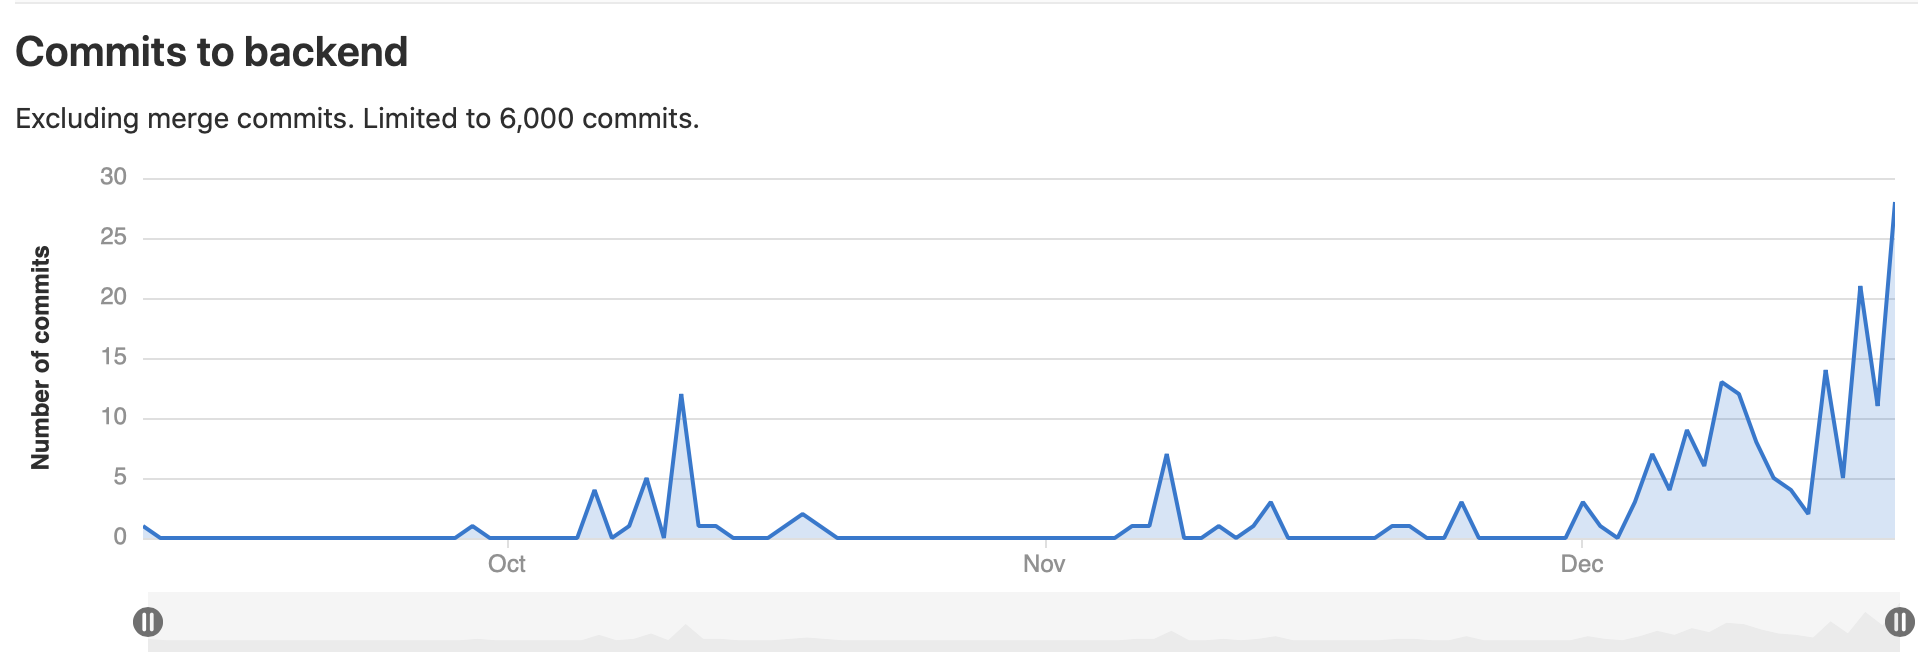
\includegraphics[width=\linewidth]{dijagrami/a.png}
			\centering
			\caption{Dijagram pregleda promjena na grani backend}
			\label{fig:ClassDiagram1}
		\end{figure}
	\begin{figure}[H]
		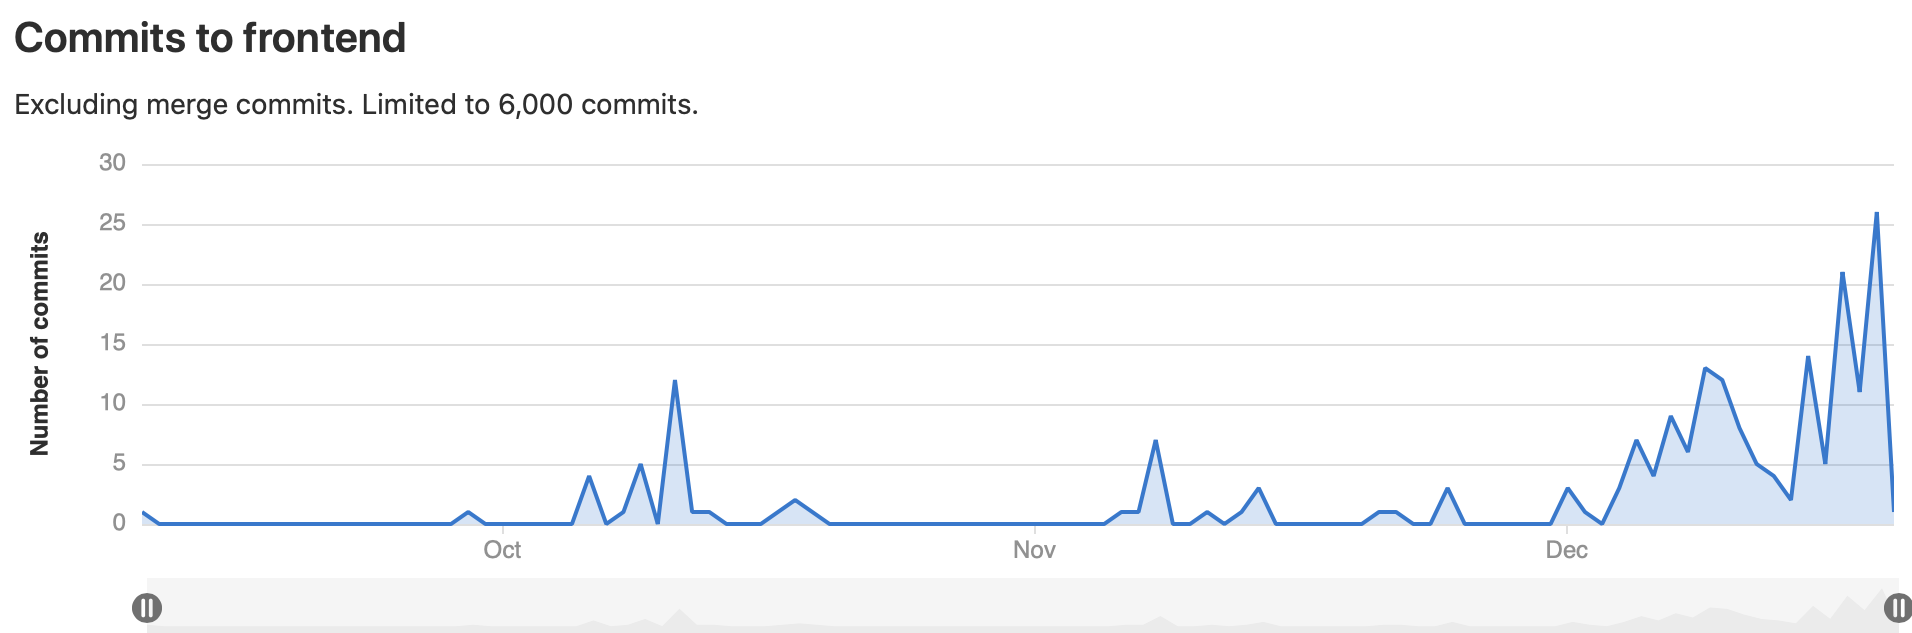
\includegraphics[width=\linewidth]{dijagrami/b.png}
		\centering
		\caption{Dijagram pregleda promjena na grani frontend}
		\label{fig:ClassDiagram1}
	\end{figure}
\begin{figure}[H]
	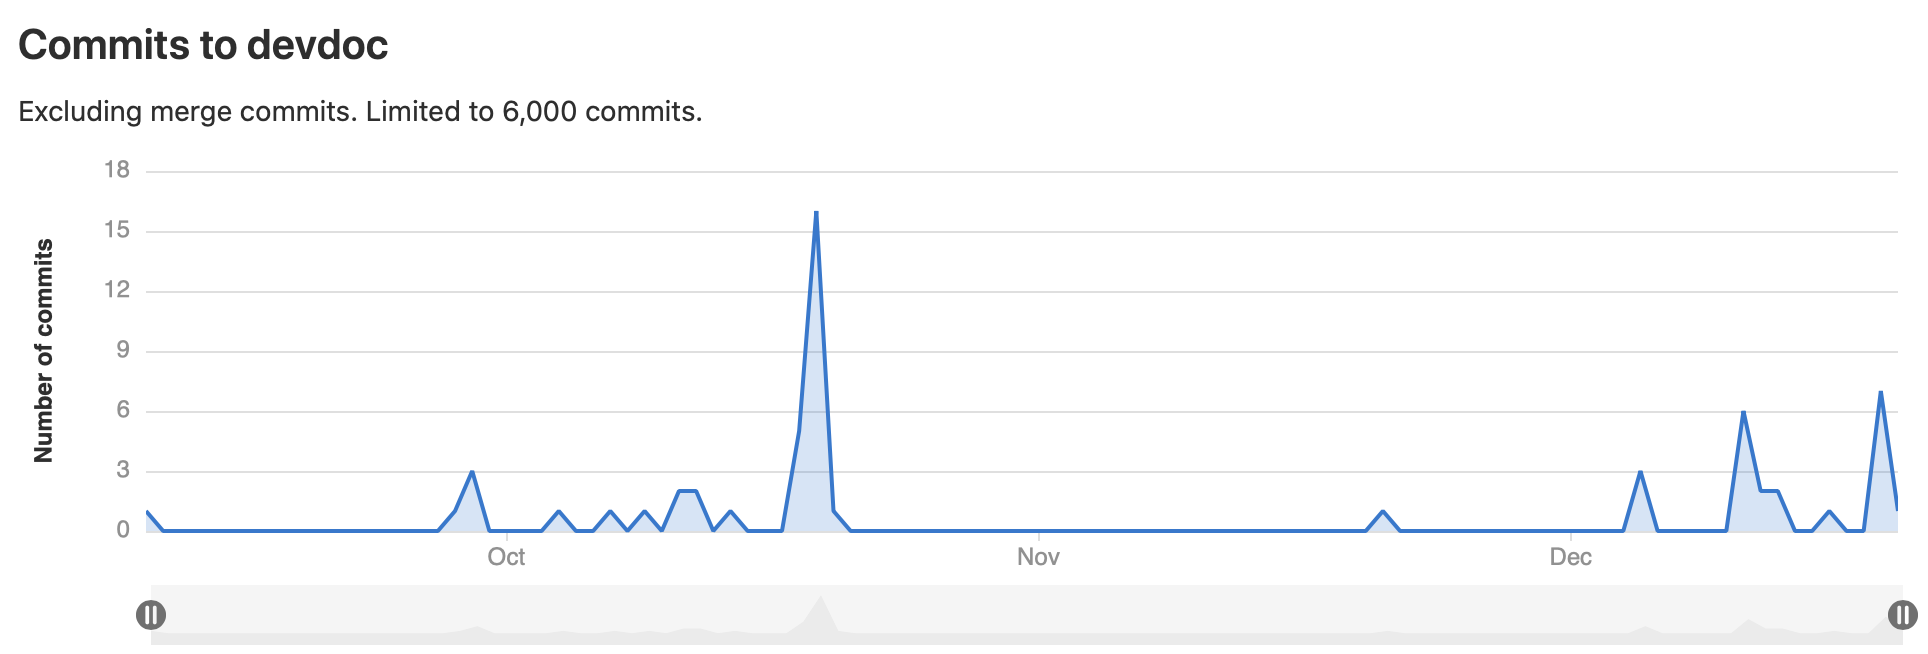
\includegraphics[width=\linewidth]{dijagrami/c.png}
	\centering
	\caption{Dijagram pregleda promjena na grani develop}
	\label{fig:ClassDiagram1}
\end{figure}
		
	